%\documentclass{article}
\documentclass[a4paper,12pt]{article}
% Seitenränder in schön für Steven
\usepackage[paper=a4paper,left=25mm,right=25mm,top=25mm,bottom=25mm]{geometry}
\usepackage{enumitem}
\usepackage{amsmath}
\usepackage{graphicx}
\usepackage{tikz}
\usepackage{titling}


% Schusterjungen und Hurenkinder bestrafen
\clubpenalty50000
\widowpenalty50000
\displaywidowpenalty=50000

% Buchstaben mit kringel drum: %
\newcommand*\mycirc[1]{%
	\begin{tikzpicture}[baseline=(C.base)]
	\node[draw,circle,inner sep=1pt](C) {#1};
	\end{tikzpicture}}

\author{Benedict Hans, Christoph Dollase, Steven Te\ss endorf}
\setlength{\droptitle}{-5em} % set the title to the top of the page

% ==========================
% ===== START HERE!! =======
% ==========================
\title{ \textbf{Problem Sheet 6}}
\setcounter{section}{6} % Nummer des Aufgabenblattes

\begin{document}	 
	\maketitle	 %Some Vodoo-magic
	
	\subsection{Modulation 2}
	\textbf{Consider the following modulation diagram.}
    
	\begin{figure}[h!]
		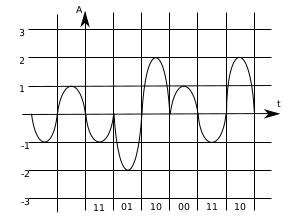
\includegraphics[width=0.4\linewidth]{modulation.png} 
    	\caption{Modulationgraph}
	\end{figure}
    
    \textbf{The signal has already been sampled and demodulated. The symbols are depicted in the 
	modulation diagram. Specify the (de-)modulation table for the applied (de-)modulation scheme.
	Sketch the corresponding constellation diagram.}

    \begin{figure}[h!] 
        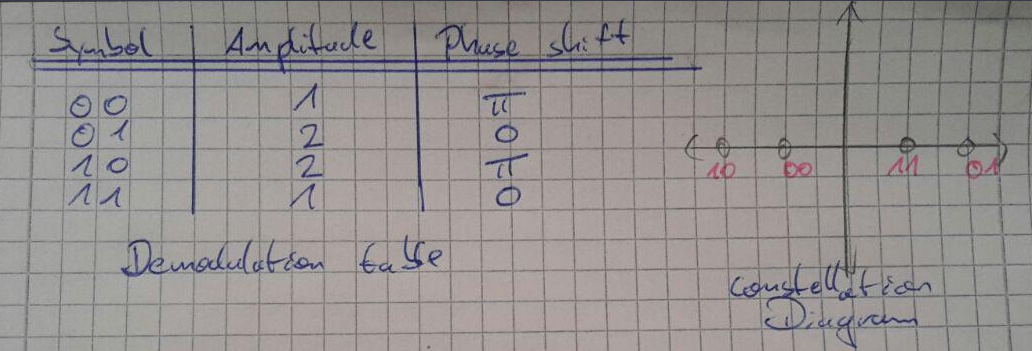
\includegraphics[width=1\linewidth]{mod_solution.png} 
	    \caption{Table and constellation diagram}
    \end{figure}
	
	\newpage
	
	\subsection{Modulation 3}
	\textbf{Modulate the bit sequence 100101111001 using a combination of amplitude and frequency
	shift keying. Each symbol shall be modulated for 1/2 T time units on the sine carrier wave.
	Use the information table in the assignment sheet.}
	
    \begin{figure}[h!] 
        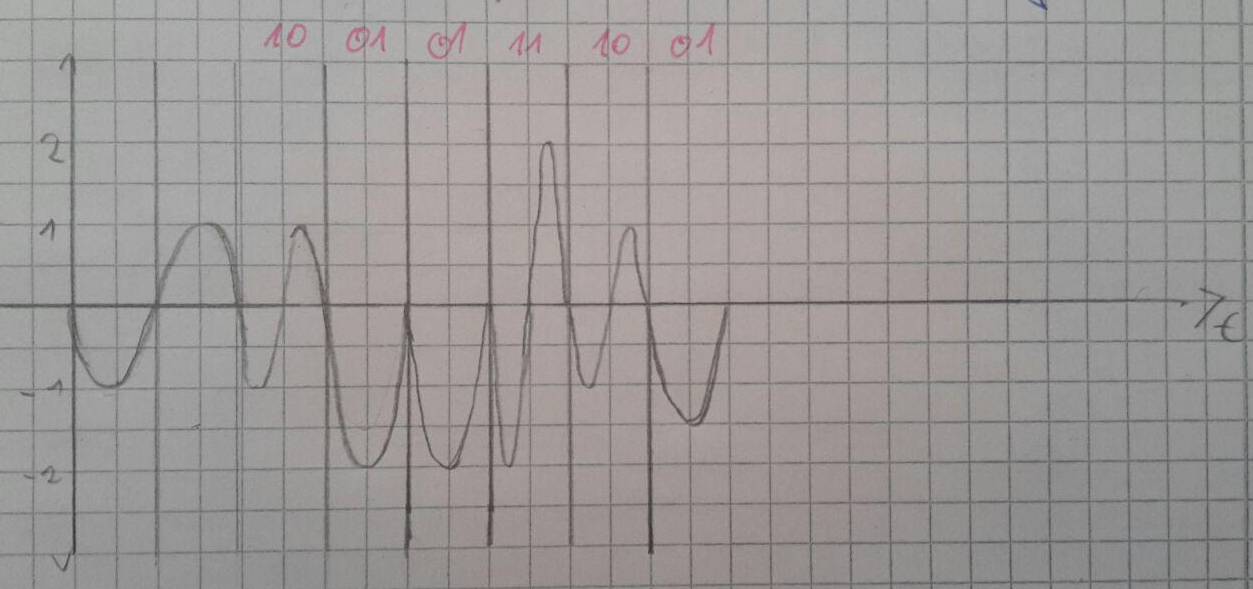
\includegraphics[width=1\linewidth]{mod_solution2.png} 
	    \caption{Modultiongraph}
    \end{figure}
	
	% Solution
	
	\subsection{title}
	\textbf{question}
	
	
	% Solution 
\end{document}

% Hier nach passiert nichts mehr, daher nutzen wir das als kleines Cheat-Sheet ;)
% ===============================================================================

% Aufzählungen (auch merhstufig):
\begin{itemize}[itemsep=0pt]
	\item 
\end{itemize}

%Bilder eifnügen:
\begin{figure}[h!] %h! sorgt dafür dass das Bild möglichst nicht woanders hingeschoben wird
	%Erklärung: [width=0.5\linewidth] -> Bild ist maximal so breit wie die Hälfte des Schriftbildes
	\includegraphics[width=0.5\linewidth]{Bildname.jpg} 
	\caption{Bildunterschrift}
\end{figure}

%Tabelle einfügen:
\begin{table}[h!] %h! sorgt dafür dass die Tabelle möglichst nicht woanders hingeschoben wird
	\caption{Tabellenüberschrift}
	%hinter {tabular}: Anzahl Spalten (c=center, l=linksbündig, r=rechtsbündig, | Spaltenstriche)
	\begin{tabular}{|c|c|c} 
		A & B & C  \\ % \\ = return (neue zeile)
		\hline % horinzontale Linie
		0 & 1 & 2
	\end{tabular}
\end{table}
